\documentclass[11pt]{article}
\usepackage{scribe}
\usepackage{graphicx}

% Uncomment the appropriate line
%\Scribe{Your name}

\Scribes{Frendy Lio Can}
\LectureDate{November 14, 2020}
\LectureTitle{Algorithms Assignment 10}

%\usepackage[mathcal]{euscript}


\begin{document}
\MakeScribeTop

%\paragraph{This is a paragraph heading} Paragraph.

%%%%%%%%%%%%%%%%%%%%%%%%%%%%%%%%
% PROBLEM 1
%%%%%%%%%%%%%%%%%%%%%%%%%%%%%%%%
\paragraph{\noindent\textbf{\LARGE{Problem 1}}}

% Start of Explaining

\begin{flushleft}
    The difference between a binary-search-tree (BST) and the min-heap property is that the BST property maintains
    an invariant where all nodes in the subtree are smaller, and all nodes in the right subtree are larger. The min-heap property only guarantees
    that the parent node is always smaller than the child node; we don't know if the left children or right children is bigger. 
    \newline
    \newline
    The min-heap property cannot be used to print out the keys of an $n$-node tree in sorted order in $O(n)$ time because we don't know
    if the left tree or right tree contains the smallest element. 
\end{flushleft}   

%%%%%%%%%%%%%%%%%%%%%%%%%%%%%%%%
% PROBLEM 2
%%%%%%%%%%%%%%%%%%%%%%%%%%%%%%%%
\paragraph{\noindent\textbf{\LARGE{Problem 2}}}

\begin{flushleft}
    Let x be a node that has two children, p be the predecessor of x, and, s be the successor of x.
    \newline
    \newline
    Lets show by contradiction that s has no left child. Suppose s has a left child. Then the values of s is greater than the value of s->left.
    This imply that the value of s->left is bigger than the value of x node. Therefore:
\end{flushleft}  
\begin{equation*}
\begin {split}
    value[s] \geq value[s \rightarrow left] \geq value[x]
\end {split}
\end{equation*}
\begin{flushleft}
    This is a contradiction as s should be the successor of x. Therefore, the successor of x cannot have a left child.
    \newline
    \newline
    Lets show by contradiction that p has no right child. Suppose p has a right child. Then the value of p is less than that value of p->right.    
    This imply that the value of p->right is less than the value of x node. Therefore:
\end{flushleft} 
\begin{equation*}
\begin {split}
    value[p] \leq value[p \rightarrow right] \leq value[x]
\end {split}
\end{equation*}
\begin{flushleft}
    This is a contradiction as p should be the predecessor of x. Therefore, the predecessor of p cannot have a right child.
\end{flushleft} 

%%%%%%%%%%%%%%%%%%%%%%%%%%%%%%%%
% PROBLEM 3
%%%%%%%%%%%%%%%%%%%%%%%%%%%%%%%%
\paragraph{\noindent\textbf{\LARGE{Problem 3}}}

\begin{flushleft}
    Worst case (Input is already sorted): $\theta(n^2)$
    \newline
    \newline
    Best case (When the tree formed is balanced): $O(nlgn)$
\end{flushleft}  


%%%%%%%%%%%%%%%%%%%%%%%%%%%%%%%%
% PROBLEM 4
%%%%%%%%%%%%%%%%%%%%%%%%%%%%%%%%
\paragraph{\noindent\textbf{\LARGE{Problem 4}}}

\begin{flushleft}
    The resulting tree is a red-black tree since the properties 1,3,4, and 5 for red-black tree are satisfied. 
\end{flushleft}

%%%%%%%%%%%%%%%%%%%%%%%%%%%%%%%%
% PROBLEM 5
%%%%%%%%%%%%%%%%%%%%%%%%%%%%%%%%
\paragraph{\noindent\textbf{\LARGE{Problem 5}}}

\begin{flushleft}
If both children are black, then the degree is 2. If one of the children is red and the others is black, then the degree is 3. If both children are red, then the degree is 4.
We can observe that the depth of the leaves of the resulting tree are the same.
\end{flushleft}    

%%%%%%%%%%%%%%%%%%%%%%%%%%%%%%%%
% PROBLEM 6
%%%%%%%%%%%%%%%%%%%%%%%%%%%%%%%%
\paragraph{\noindent\textbf{\LARGE{Problem 6}}}
\begin{flushleft}
    For a red-black tree, we know that every simple path from node $x$ to a descendant leaf, the same number of black nodes and
red nodes do not happen next to each other.
    \newline
    \newline
    Thus, we can conclude that the shortest path from node $n$ to a descendant leaf will have all nodes of color black.
    We can also conclude that the longest path will be a path with alternating black and red nodes.
    \newline
    \newline
    Since all leaf must be black, the longest path will have the same number of red and black nodes. It will have $2* ($ number of black nodes $)$, where the number of black nodes is equal
    to the shortest path. 
\end{flushleft}    
    

%%%%%%%%%%%%%%%%%%%%%%%%%%%%%%%%
% PROBLEM 7
%%%%%%%%%%%%%%%%%%%%%%%%%%%%%%%%
\paragraph{\noindent\textbf{\LARGE{Problem 7}}}
\begin{flushleft}
    Lets consider a $n$-node binary tree where will be transform it into a right-going chain. Let the root and all its right children be elements of the chain.
    For any node $x$ which is a left child of a node on the chain, a single right rotation on the parent of $x$ will add that node to the chain and not remove 
    any elements from the chain. Therefore, we can transform the arbitrary $n-$node binary search tree to a right-going chain with at most $n-1$ right  rotations.
    \newline
    \newline
    In order to convert the right-going chain into any other arbitrary $n-$ node binary search tree will take also $n-1$ rotations. Therefore, the time complexity is $O(2n-2) = O(n)$.
\end{flushleft}

%%%%%%%%%%%%%%%%%%%%%%%%%%%%%%%%
% PROBLEM 8
%%%%%%%%%%%%%%%%%%%%%%%%%%%%%%%%
\paragraph{\noindent\textbf{\LARGE{Problem 8}}}
\begin{flushleft}
\begin{figure}[htbp]
    \centerline{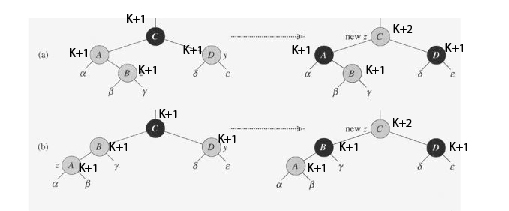
\includegraphics[scale=.5]{pict1.JPG}}
\end{figure}
\begin{figure}[htbp]
    \centerline{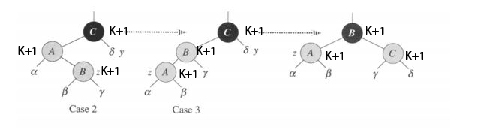
\includegraphics[scale=.5]{pict2.JPG}}
\end{figure}
    
\end{flushleft}

%%%%%%%%%%%%%%%%%%%%%%%%%%%%%%%%
% PROBLEM 9
%%%%%%%%%%%%%%%%%%%%%%%%%%%%%%%%
\paragraph{\noindent\textbf{\LARGE{Problem 9}}}
\begin{flushleft}
    Using $OS-SELECT(x,i)$ and $OS-RANK(T,x)$ from the CLRS book page 341 and 342.
    The desired result is $OS-SELECT(T, OS-RANK(T, x) + i)$. 
    This has runtime $O(h)$, where h is the height of the tree. We know by the properties of red black trees that
    $h = lgn \Rightarrow O(lgn)$
\end{flushleft}

%%%%%%%%%%%%%%%%%%%%%%%%%%%%%%%%
% PROBLEM 10
%%%%%%%%%%%%%%%%%%%%%%%%%%%%%%%%
\paragraph{\noindent\textbf{\LARGE{Problem 10}}}
\begin{flushleft}
    We can use the $INTERVAL-SEARCH(T,i)$ algorithm from the CLRS book (page 351), 
    but, instead of breaking out of the loop as soon as we have an overlap, we just keep track of the overlap that has the minimum low endpoint, and continue the loop. After the loop terminates, we return the overlap stored.
    \newline
    \newline
    Thus, it would look something like this:
    \newline
    \newline
    INTERVAL-SEARCH-MODIFIED(T, i) \\
    x = T.root \\
    interval = T.nil \\
    while x $\neq$ T.nil:\\
    \quad $\backslash$$\backslash$ keep track of overlap \\
    \quad if not (i.high $\leq$ x.left or x.right $\leq$ i.low) \\
    \quad \quad if interval == T.nil or interval.right > x.right \\
    \quad \quad \quad interval = x \\
    \quad if x.left $\neq$ T.nil and x.left.max $\geq$ i.low \\
    \quad \quad x = x.left\\
    \quad else \\
    \quad \quad x = x.right\\
   return interval    
\end{flushleft}


\end{document}


